\providecommand{\main}{../../../..}
\documentclass[\main/dresen_thesis.tex]{subfiles}
  \renewcommand{\thisPath}{\main/chapters/monolayers/paracrystal/verticalStructure}

\begin{document}
  As discussed in \refch{sec:theoreticalBackground:scattering:reflectometry}, reflectometry is an excellent method to resolve the vertical structure of a sample.
  X-ray reflectometry yields information on the average electron density distribution with respect to the vertical axis, whereas neutron reflectometry yields information on the nuclear structure and in case of polarized neutrons additionally on the spin density.

  Parrats recursive method is most efficient for samples that have in average a constant lateral scattering length density (SLD) for relative large parts of their height, as it models the density profile using slabs and interfacial roughness as parameters.
  This is beneficial for the case of nanocubes in a square lattice, as they can be described by very few parameters.

  \begin{figure}[tb]
    \centering
    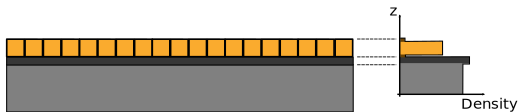
\includegraphics{monolayer_structure_verticalModel}
    \caption{\label{fig:monolayers:structure:verticalModel}Model for a square array of nanocubes depicted as cartoon of the cross-section (left) and the expected resulted shape of the vertical density structure (right).}
  \end{figure}

  The model that is used in this section to discuss reflectometry data is depicted schematically in \reffig{fig:monolayers:structure:verticalModel}.
  The lower grey area represents the silicon substrate with the possibility of a silicion dioxide (\ch{SiO2}) layer on top.
  The average lateral density of a square array layer is modeled by a single slab, with lower density slabs for possible oleic acid spacers around it.
  In general, it can not be excluded that parts of a real monolayer sample have small islands of a second layer on top.
  Therefore the model includes a second slab for the nanoparticles, which is also surrounded by oleic acid spacer.
  The oleic acid spacer in between the particles is modeled as one slab, as it is reasonable to assume that the oleic acid chains mix and become indistinguishable on average.
  Due to the three different surroundings for each oleic acid layer (silicon/particle, particle/particle, particle/air), the density and and thickness of each is allowed to vary independently.
  And at last, which is not depicted in \reffig{fig:monolayers:structure:verticalModel}, the interfaces are not clear cuts in the vertical plane but have a certain interfacial roughness, which are treated by roughness parameters in the model for each type of interface.

  In total the ideal model has $17$ parameters: the edge length and SLD of the nanocubes, the two packing densities of the layers, the $6$ parameters to describe the three oleic acid layers, the SLD and thickness of the \ch{SiO2} layer, the SLD of the silicon material and $4$ roughness parameters for the interfaces \ch{Si}/ch{SiO2}, \ch{SiO2}/oleic acid, oleic acid/nanocube and oleic acid/air.
  A number of parameters can be fixed by complementary experiments to reduce the number of parameters.
  The edge length and SLD of the nanocubes are determined by small-angle scattering experiments.
  The substrate properties and check for a \ch{SiO2} layer is determined by measuring an empty wafer, determining the \ch{Si} SLD, the \ch{SiO2} thickness and SLD and the \ch{Si}/\ch{SiO2} roughness.
  Thus the number of parameters for the model can be reduced $11$ parameters, additional to the instrumental property parameters that need to be considered.

  The x-ray reflectometry data has been measured on an Bruker D8 instrument at the \textsc{Forschungszentrum J\"ulich}, which is described in \refapp{app:additionalExperimentalTechniques:xrr}.
  After definition of the model and its parameters, the parameter values are refined by applying the Levenberg-Marquardt algorithm %add citation
  , to minimize the $\chi^2$ value, which is defined here as
  \begin{align}
    \chi^2 \eq \sum_{q_i} \biggl( \frac{\log(I) - \log(I_\mathrm{model})}{\sigma_i} I\biggr)^2,
  \end{align}
  to minimize the quadratic distance on the logarithmic scale.

  \begin{figure}[tb]
    \centering
    \includegraphics{monolayers_VerticalStructure_SiliconSubstrate_XRR}
    \includegraphics{monolayers_VerticalStructure_SiliconSiliconDioxide_XRR}
    \caption{\label{fig:monolayers:structure:emptySiliconWafer}Model for a square array of nanocubes depicted as cartoon of the cross-section (left) and the expected resulted shape of the vertical density structure (right).}
  \end{figure}
  The x-ray reflectometry measurement of an empty wafer, shown in \reffig{fig:monolayers:structure:emptySiliconWafer}, is already very well described by a simple model of only a silicon substrate with an SLD of $\mathrm{SLD}_{\ch{Si}} \eq 19.687(8) \cdot \unit{10^{-6} \angstrom^{-2}}$ and an surface roughness of $\sigma \eq 0.932(8)\unit{nm}$.% \chi^2 \eq 128.
  Adding another slab as shown in the right image, to allow for a silicon dioxide layer on top does not significantly improve the $\chi^2$ value.
  In this case, the constant background parameter that is implemented to account for background noise, reduces from $I_{bg} \eq 3 \cdot 10^{-6}$ to $0$, while a second layer with low SLD rises.
  Also in comparison to the literature value of silicon dioxide ($\mathrm{SLD}_{\ch{SiO2}} \eq 22.677  \cdot \unit{10^{-6} \angstrom^{-2}}$).
  As the SLD of the second layer here is significantly lower, this speaks either an incomplete or highly porous silicon dioxide

  In the case of x-rays ($\lambda \eq 1.54 \unit{\angstrom}$), the contrast in SLD between bulk silicon dioxide () and silicon ($\mathrm{SLD}_{\ch{Si}} \eq 20.053 \cdot \unit{10^{-6} \angstrom^{-2}}$) 



\end{document}